\documentclass[12pt, a4paper]{article}

\usepackage[utf8]{inputenc}
\usepackage[T2A]{fontenc}
\usepackage[russian]{babel}
\usepackage[dvips]{graphicx}
\usepackage{float}
\usepackage[oglav,spisok,boldsect,eqwhole,figwhole,hyperref,hyperprint,remarks,greekit]{./style/fn2kursstyle}
\graphicspath{{./style/}{./figures/}}

\usepackage{multirow}
\usepackage{supertabular}
\usepackage{multicol}
\usepackage{hhline}
\usepackage{listings}
\usepackage{color}
\usepackage{adjustbox}

\definecolor{dkgreen}{rgb}{0,0.6,0}
\definecolor{gray}{rgb}{0.5,0.5,0.5}
\definecolor{mauve}{rgb}{0.58,0,0.82}

\lstset{frame=tb,
	language=Python,
	aboveskip=0.5mm,
	belowskip=0.5mm,
	showstringspaces=false,
	columns=flexible,
	basicstyle={\small},
	numbers=left,
	numberstyle=\tiny\color{gray},
	keywordstyle=\color{red},
	commentstyle=\color{dkgreen},
	stringstyle=\color{mauve},
	breaklines=true,
	breakatwhitespace=true,
	tabsize=2
}
\newcommand\thh[1]{\text{\mathversion{bold}${#1}$}}
\renewcommand{\labelenumi}{\theenumi)}
\renewcommand{\labelenumi}{\theenumi)}


\newcommand{\opr}{\textbf{\underline{{Опр.}}}\quad}
\newcommand{\theorem}{\textbf{\underline{{Теор.}}}\quad}
\renewcommand{\phi}{\varphi}
\renewcommand{\k}[1]{\textbf{\textit{#1}}}
\newcommand{\widecheck}[1]{\check{#1}}
\renewcommand{\kappa}{\varkappa}

\newcounter{mycounter}
\newcommand{\question}[1]{%
	\stepcounter{mycounter}%
	\textbf{\themycounter}.  %
	\textbf{\textit{#1}}
	
}
\newcommand{\down}[1]{\widecheck{#1}}
\newcommand{\pon}[1]{\mathop {#1}\limits^ \circ}
\newcommand{\rusg}{\text{Г}}

\usepackage[a4paper, margin=1.5cm]{geometry} % Устанавливаем узкие поля по 1 см


\begin{document}
	\section-{Краткое изложение решения задачи регрессии с помощью нейронной сети}
	\begin{center}
		\centering{Автор: Климов О.Д., ФН2-71Б}
	\end{center}
	
	\section{Введение}
	Данная работа представляет собой некоторое математическое обоснование тех методов, которые используются автором для решения задачи регрессии объектов на изображении.\\ В данном случае стоит задача: на ч/б изображении определенной размерности есть график функции $f(x) = C = const$, где $C \in [a, b]$. Параметры $a$ и $b$, считаем заданными. Масштаб графика по обеим осям считаем постоянным и в диапазоне $[0, 1]$. 
	
	Необходимо:
	\begin{enumerate} 
		\item По изображению графика определить параметр $A$. 
		\item Пусть изображение задано не прямой, а точками некого численного решения задачи, и имеется небольшая погрешность. Необходимо также определить параметр $A$. 
		\item Пусть есть изображение, где параметр $A$ лежит вне $[a, b]$. Определить параметр A.
	\end{enumerate}
	
	Для решения задачи будем использовать нейронную сеть, которая будет по изображению выдавать значение параметра. Далее будут приведены соответствующая теория и анализ результатов. Решение задачи приводит и к решению ее более сложных случаев, где, например, может понадобиться распознать и тип функции и ее параметры.
	
	\section{Понятие регрессии и ее отличие от классификации}
	Задачи нейронных сетей обычно делятся на задачи классификации и регрессии.\\
	В задаче \textbf{классификации} нужно поданный на вход объект определить в один из(обычно конечного числа) классов, например, разделить фотографии животных на кошек, собак, лошадей и т.п.; или по фотографии человеческого лица понять, кто из определенного круга лиц на ней изображен. Типичная задача классификации — это разметка слов по частям речи. \\
	В задаче \textbf{регрессии} нужно предсказать значение некой функции, у которой обычно может быть бесконечно много разных значений. Например,по росту человека предсказать его вес, сделать прогноз завтрашней погоды, предсказать цену акции или выделить на фотографии прямоугольник, в котором находится человеческое лицо — сделать это необходимо, чтобы затем эти прямоугольники подать на вход упомянутому выше классификатору\cite[см. стр.~19]{1}.
	
 	Позже будет показана структура нейронной сети и будет понятно, что итогом работы программы нейронной сети является последний выходной слой. В случае задачи классификации мы бы специально подбирали структуру сети так, чтобы значение одного из нейронов в сети было заметно выше других. Тогда результатом всего алгоритма классификации была метка, которая назначена этому нейрону, то есть мы бы выбрали определенный класс. В случае задачи регрессии числовые значения нейронов последнего слоя являются значениями соответствующих им параметров решения задачи. То есть, например, в нашей задаче мы распознаем параметр $A$, а значит последний слой будет иметь только один нейрон, который и будет результатом всего алгоритма.
	\section{Полносвязная нейронная сеть}
	Начнем с наиболее простого алгоритма сети--- полносвязной нейронной сети(Fully Connected Neural Network, FCNN), и рассмотрим основную структуру сети. 
	%, хотя они являются не самыми эффективными при работе с пространственными зависимостями на изображении. Позже рассмотрим более сложный подход --- сверточную нейронную сеть (Convolutional Neural Network, CNN), относящуюся уже к глубокому обучению. 
	

	\subsection{Нейрон}
	Пусть представляет собой единицу обработки информации в нейронной сети. На показана модель нейрона, лежащего в основе искусственных нейронных сетей. В этой модели выделяют три основных элемента\cite[см. стр.~40-41]{2}.:
	\begin{itemize}
		\item \textbf{Набор связей}, каждый из которых характеризуется своим весом(силой). В частности, сигнал $x_j$ на входе связи $j$, связанного с нейронном $k$, умножается на вес $w_{kj}$(первый индекс относится к рассматриваемому нейрону, а второй ко входному окончанию связи). Вес может иметь как положительные так и отрицательные значения.
		\item \textbf{Сумматор} складывает входные сигналы, взвешенные относительно соответствующих связей нейрона. Эту операцию можно описать как линейную комбинацию.
		\item \textbf{Функция активации} ограничивает амплитуду выходного сигнала нейрона. Обычно нормализованный диапазон амплитуд выхода нейрона лежит в интервале $[0, 1]$ или $[-1, 1]$.
		\item \textbf{Пороговый элемент} $b_k$, который отражает увеличение или уменьшение входного сигнала на функцию активации.
	\end{itemize}
	
	\begin{figure}[!h]
		\centering
		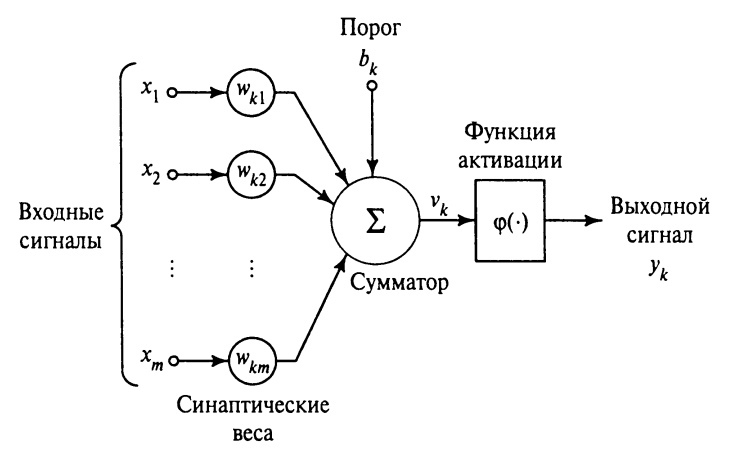
\includegraphics[width=0.8\linewidth]{neiron}
		\caption{Нелинейная модель нейрона}
		\label{neiron}
	\end{figure}
	\newpage
	В математическом представлении функционирование нейрона $k$ можно описать следующей парой уравнений
	\begin{equation*}
		y_k = \phi(u_k + b_k), \quad u_k = \sum_{j = 1}^{m} w_{kj}x_j 
	\end{equation*}
	где $x_1, x_2, \dots, x_m$ --- входные сигналы,
	 $w_{k1}, w_{k2}, \dots, w_{km}$ --- веса связей нейрона $k$, \\
	 $u_k $ --- линейная комбинация входных воздействий,
	 $b_k$ --- порог,\\
	 $ \phi(\dot) $ --- функция активации,
	 $ y_k $ --- выходной сигнал.
	 
	Использование порога $b_k$ обеспечивает эффект афинного преобразования выхода линейного сумматора $u_k$. В частности, в зависимости от того, какое значение принимает порог,  положительное или отрицательное, можно двигать значения выхода нейрона. Обознчим $w_{k0} = b_k$ и преобразуем модель к следующему виду
	\begin{equation*}
		y_k = \phi(v_k), \quad v_k = \sum_{j = 0}^{m} w_{kj}x_j 
	\end{equation*}
	\subsection{Слои нейронов}
	В многослойной нейронной сети нейроны располагаются по слоям. В простейшем случае в такой сети существует входной слой узлов источника, информация от которого предается на выходной слой нейроной(вычислительные узлы). Такая сеть называется сетью прямого распространения. 
	
	\textbf{Полносвязная нейронная сеть (FCNN)} — это сеть, в которой каждый нейрон одного слоя соединен со всеми нейронами следующего слоя. Она характеризуется наличием одного(соответствующей модели перцептрон) или нескольких скрытых слоев, узлы которых называются скрытыми нейронами. Их Функция заключается в посредничестве между внешним входным сигналом и выходом нейронной сети. Добавляя скрытые слои мы можем выделить статистики высокого порядка. Такая сеть способна выделять глобальные свойства данных с помощью локальных соединений за счет повышенного уровня взаимодействия нейронов.
	
	\begin{figure}[!h]
		\centering
		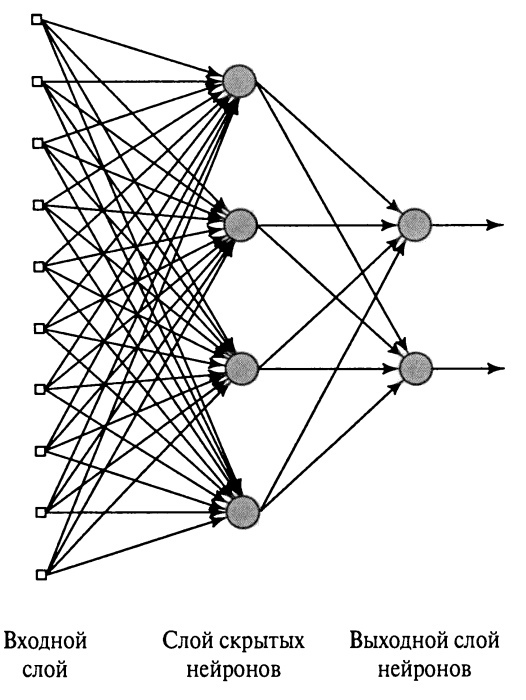
\includegraphics[width=0.3\linewidth]{web}
		\caption{Полносвязная сеть с одним скрытым слоем}
		\label{neiron}
	\end{figure}
	
	\section{Предварительная обработка изображений}
	В исходной задаче есть известные нам данные --- изображение графика и некоторая информация о нем. В эту информацию входит: тип функции на графике ($f(x) = C $), размер изображения, масштаб осей(т.е. область определения функции на изображении), формат файла изображения(пусть будет $*.png$).
	
	Как было показано выше, входными данными в алгоритм нейронной сети является вектор числовых значений. Поэтому мы можем преобразовать наше изображение к корректный для будущей обработки формат. Сделаем это следующим образом:
	
	\begin{enumerate}
		\item Черно-белое изображение в формате $*.png$ представляет собой двумерный массив чисел от $[0, 255]$. Каждый элемент массива является значением яркости соответствующего пикселя. Поэтому представим файл двумерного массива в языке программирования Python. 
		\item Пересоберем двумерный массив в одномерный, соединив все строки друг за другом.
		\item Поделим каждый элемент массива на $255$, чтобы значения находились в диапазоне $[0, 1]$
	\end{enumerate}
	
	Такие действия проводятся с изображениями в каждом случае перед подачей в алгоритм нейронной сети. При наличии цветового шума можно воспользоваться соответствующими алгоритмами и перевести любое изображение в черно-белый формат, при этом оставить только наиболее яркие значения цветов, назначив им максимальное числовое значение. После мы получим вектор с двумя возможными значениями: $0$ или $1$.

	
	
	\section{Обучение полносвязной сети}
	
	Нейронная сеть состоит слоев и связей между ними. Основными параметрами сети являются именно коэффициенты связей $w$, которые мы и будем изменять для того, чтобы настроить сеть выдавать наиболее верный результат. Часто эти параметры называются весами.
	
	Процесс обучения предполагает следующую последовательность событий, называемую алгоритмом обучения\cite[см. стр.~87]{2}.:
	
	\begin{enumerate}
		\item В сеть поступает вектор числовых значений(стимул) из специально подготовленного тренировочного набора данных
		\item В результате этого, на основе некоторого алгоритма, изменяются параметры самой сети
		\item После изменения внутренней структуры нейронная сеть выдает уже иной результат
		\item
	\end{enumerate}
	
	В нашем случае алгоритмом, который будет использоваться для корректировки весов будем использовать метод обратного распространения ошибки.
	
	\section{Пример решения задачи регрессии}
	Для построения вышеописанных алгоритмов на языке программирования Python воспользуемся удобной и практичной библиотекой машинного обучения TensorFlow, которая разрабатывается компанией Google. Библиотека представляет весь спектр инструментов для разработки полного цикла работы программы. 
	
	Пусть у нас уже есть некоторое количество тренировочных и тестовых наборов изображений, которые можно несложно создать с помощью математического пакета, например Wolfram Mathematica. В нашем случае наборы тестовых и тренировочных изображений $64*64$ пикс. состоят из 21 штук, причем имя файла соответствует значению параметра $C$ на изображении.
	
	С помощью функции $tf.Dataset$ создадим объект, который будет содержать в себе все изображения, метки и взаимосвязь между ними. Данный объект понадобиться для подачи на вход алгоритму сети. На изображении \ref{images} показан используемый набор данных.
	

	
	\begin{figure}[!h]
		\centering
		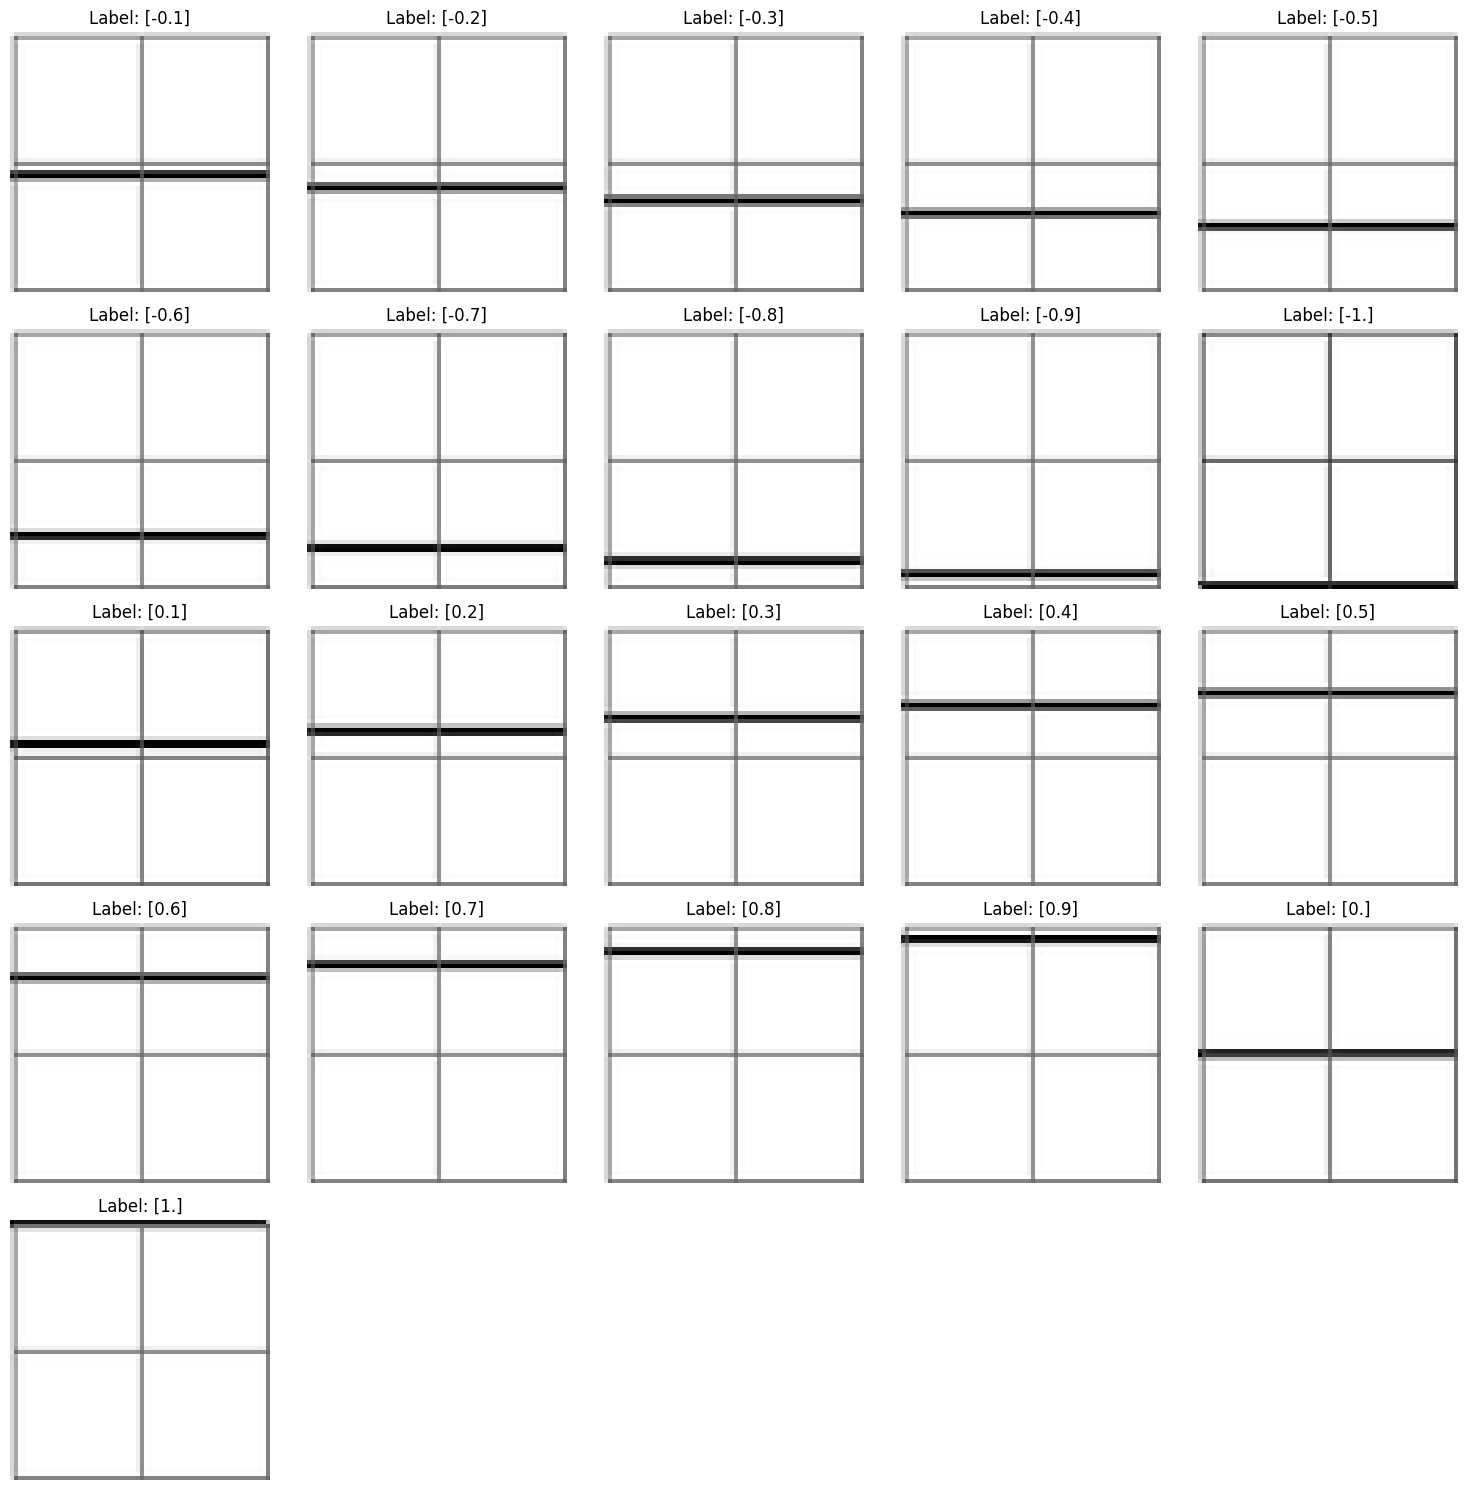
\includegraphics[width=1\linewidth]{output}
		\caption{Тренировочный набор данных с соответствующими метками (метка соответствует значению параметру $C$)}
		\label{images}
	\end{figure} 
	\newpage
	
	Саму модель сети определим следующим образом:
	\begin{figure}[!h]
		\centering
		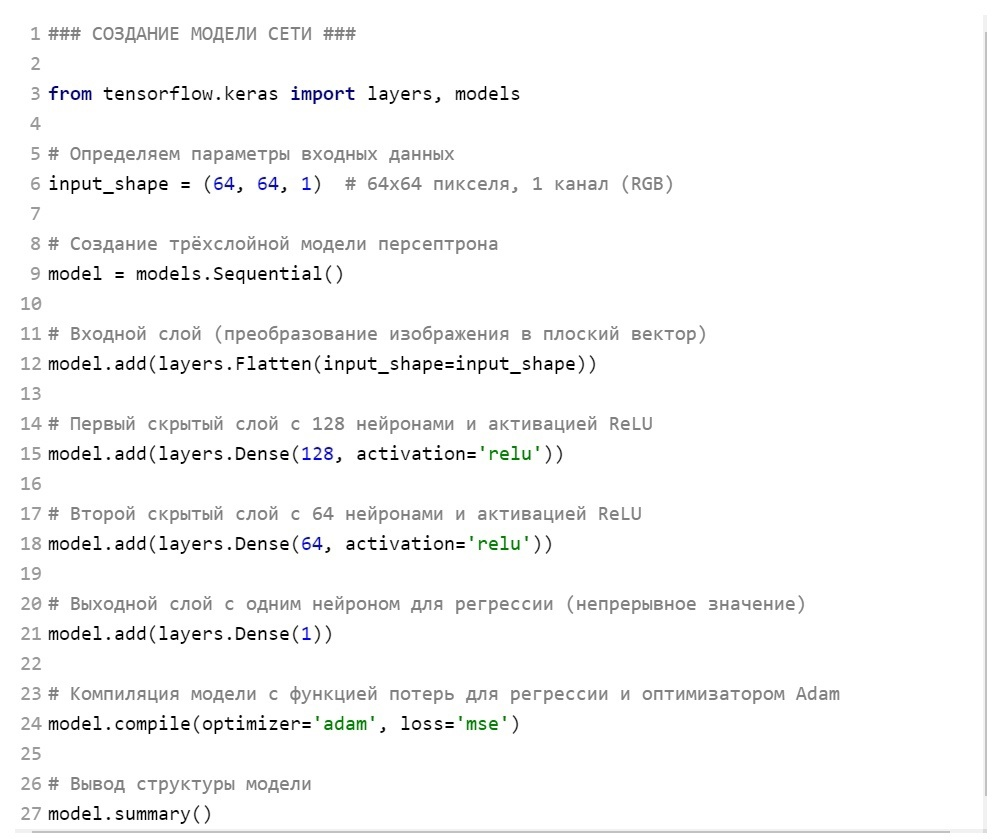
\includegraphics[width=1\linewidth]{model.jpg}
		\caption{Тренировочный набор данных с соответствующими метками (метка соответствует значению параметру $C$)}
		\label{model}
	\end{figure} 
	
	Сначала мы определяем параметры входных данных, такие как размеры входного изображения, количество каналов цветов. Создаем объект $model$, который является стандартным объектом последовательной сети в библиотеке TensorFlow. Далее мы можем добавлять в эту сеть слои. Установим два скрытых слоя по $128$ и $64$ нейрона соответственно. На выходе поставим одно непрерывное значение. Для обучения модели также можем использовать встроенный в библиотеку усовершенствованный алгоритм стохастического градиентного спуска adam. Для определения ошибки вывода нейронной сети будем использовать функцию среднеквадратичной ошибки.
	
	Далее будем обучать модель на тренировочном наборе определенное количество раз, пока не придем к наилучшему результату. Библиотека позволяет во время обучения сохранять версию модели с наилучшим результатом. Такое полезно в связи с тем, что модель может переобучиться и с продолжением обучения выдавать плохие результаты. Обучение сети измеряется в эпохах и соответствует количеству раз, сколько был подан обучающий набор данных.
	
	Для нашей модели с 2 скрытыми слоями понадобилось около 35 эпох для достижения наилучшего результата. Теперь можем протестировать сеть на тренировочных и тестовых данных. 
	
	К сожалению результаты получились неутешительными и полносвязная нейронная сеть не справляется с задачей. На изображениях \ref{train} и \ref{test} показаны результаты анализа работы сети в виде графиков. По горизонтальной оси отложено истинное значение параметра $C$, а по вертикальной оси его значение, предсказанное сетью. Из графиков можно сделать вывод о большой погрешности предлагаемого метода.
	
	\begin{figure}[!h]
		\centering
		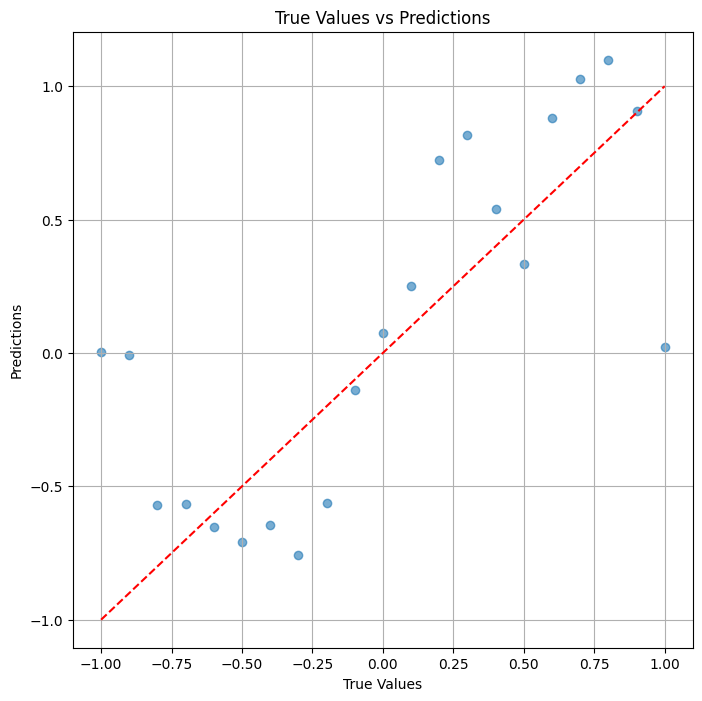
\includegraphics[width=1\linewidth]{test_output}
		\caption{Результаты работы алгоритма на тренировочных данных}
		\label{train}
	\end{figure}
	
	\begin{figure}[!h]
		\centering
		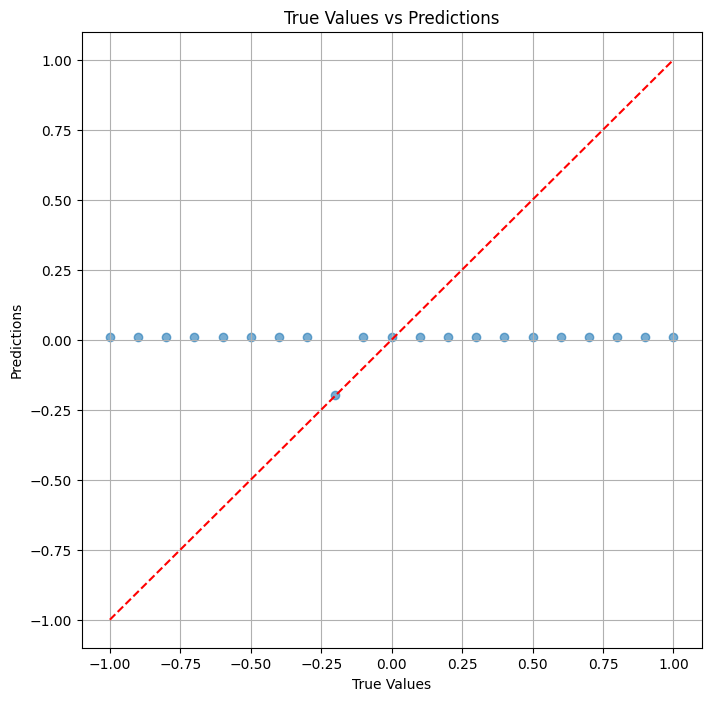
\includegraphics[width=1\linewidth]{train_output}
		\caption{Результаты работы алгоритма на тестовых данных данных}
		\label{test}
	\end{figure}

	
	\section{Проблемы и решения}
	Для достижения наилучшего результата при работе с изображениями следует использовать сверточные сети со специальными слоями. Также следует увеличить выборку изображений, а также обучать и на дополнительных наборах с погрешностями в графике. Тем самым возможно уменьшить ошибку сети.
		
	\newpage
	\begin{thebibliography}{10}
	\bibitem{1} Николенко С. Кадурин А. Архангельская Е. Глубокое обучение. --- СПб.: Питер, 2024. --- 480 с.: ил. --- (Серия "Библиотека программиста").
	\bibitem{2} Хайкин, Саймон Нейронные сети: полный курс 2-е издание. Пер. с англ. --- М. : Издательский дом "Вильямс", 2006. --- 1104 с. : ил. --- Парал. тит. англ.
	\bibitem{3} Селянкин В.В. Компьютерное зрение. Анализ и обработка изображений: учебное пособие для вузов / В.В. Селянкин --- 2-е изд., стер. --- Санкт-Петербург : Лань, 2021. --- 152с.: ил. --- Текст: непосредственный.
	\end{thebibliography}
\end{document}

	
